 % /* Copyright (c) 2015  Tizian Zeltner, ETH Zurich
 % * 
 % * Permission is hereby granted, free of charge, to any person obtaining a copy
 % * of this software and associated documentation files (the "Software"), to deal
 % * in the Software without restriction, including without limitation the rights
 % * to use, copy, modify, merge, publish, distribute, sublicense, and/or sell
 % * copies of the Software, and to permit persons to whom the Software is
 % * furnished to do so, subject to the following conditions:
 % * 
 % * The above copyright notice and this permission notice shall be included in
 % * all copies or substantial portions of the Software.
 % * 
 % * THE SOFTWARE IS PROVIDED "AS IS", WITHOUT WARRANTY OF ANY KIND, EXPRESS OR
 % * IMPLIED, INCLUDING BUT NOT LIMITED TO THE WARRANTIES OF MERCHANTABILITY,
 % * FITNESS FOR A PARTICULAR PURPOSE AND NONINFRINGEMENT. IN NO EVENT SHALL THE
 % * AUTHORS OR COPYRIGHT HOLDERS BE LIABLE FOR ANY CLAIM, DAMAGES OR OTHER
 % * LIABILITY, WHETHER IN AN ACTION OF CONTRACT, TORT OR OTHERWISE, ARISING FROM,
 % * OUT OF OR IN CONNECTION WITH THE SOFTWARE OR THE USE OR OTHER DEALINGS IN
 % * THE SOFTWARE.
 % */

\documentclass[a4paper]{article}

\usepackage[utf8]{inputenc}
\usepackage{geometry}
\usepackage{lastpage}
\usepackage{extramarks}
\usepackage{subfigure}
\usepackage{fancyhdr}
\usepackage{listings}
\usepackage{color}
\usepackage{graphicx}
\usepackage{pdfpages}

\definecolor{mygreen}{rgb}{0,0.6,0}

\lstset{
basicstyle=\footnotesize,
language = [Sharp]C,
commentstyle=\color{mygreen},
keywordstyle=\color{blue},
tabsize=4,
frame=single
}

\pagestyle{fancy}


\textheight=9.0in

\lhead{AR Treasure Hunt Hackathon}
\rhead{}
\cfoot{Page\ \thepage\ of\ \protect\pageref{LastPage}}

\usepackage[boxed]{algorithm}
\usepackage{algorithmic}

\usepackage{amsmath}

\linespread{1.1}
\setlength\parindent{0pt}
\renewcommand{\vec}[1]{\mathbf{#1}}



\begin{document}

\title{\vspace{-2em}Puzzle Creation for AR Treasure Hunt
\vspace{-2em}}
\author{}
\date{}
\maketitle
\thispagestyle{fancy}

\begin{figure}[h]
	\centering
	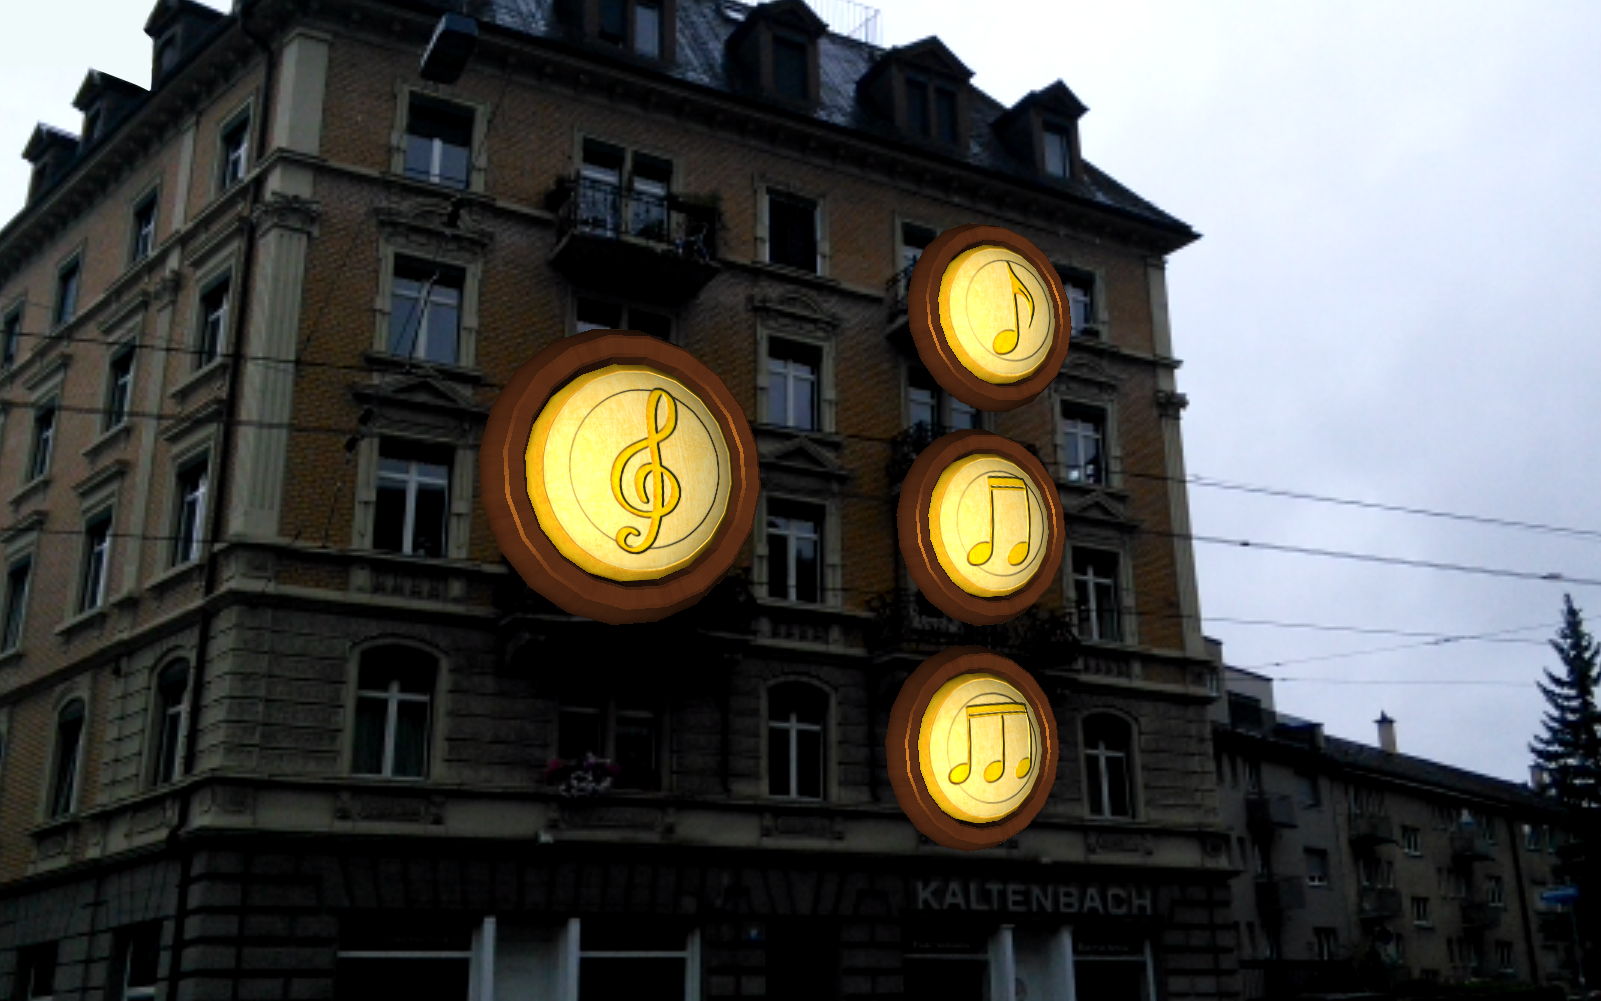
\includegraphics[width=0.8\textwidth]{figures/title}
\end{figure}


\section{About AR Treasure Hunt}

AR Treasure Hunt is a City-Wide Augmented Reality game for mobile devices.\\

Players start at a predefined starting location and then visit multiple locations in a part of Zurich. To find the locations, written clue texts have to be followed that contain directions from the last location.\\

At every location, a small puzzle (or mini-game) is virtually overlaid on a building facade with Augmented Reality. Players have to use the camera in the device to find and solve the puzzle.\\

Solving a puzzle unlocks the next chapter of the game and with it the description to find the next location. The treasure is found after solving the puzzle at the last location.

\section{Software}

In this project, the Unity 3D Game Engine is used. You can download the newest free version at http://unity3d.com/unity/download.\\

The provided templates include the Vuforia Unity Extension by Qualcomm for Augmented Reality marker tracking.

\newpage

\section{Creating your own chapter}

These steps describe how a chapter with a very simple puzzle can be added to the game. You can either follow them or open the \textit{THTemplate1} Unity package in a new Unity project for the finished version.\\

\textbf{1.} Create a new Unity project and import the \textit{THTemplateEmpty} Unity package. Open the \textit{TreasureHunt} scene from the \textit{Scenes} folder.
	
Starting the game now only shows an empty template without any chapters.\\
	
\textbf{2.} The \textit{Prefabs} folder contains some pre-built game object to use. Drag a \textit{MyChapter} prefab from the folder to the project hierarchy. Set it up as a child of the \textit{Quest} game object.\\
	
\textit{Quest} has the \texttt{QuestManager} script attached to it. Set the number of chapter game objects and drag the \textit{MyChapter} game object into the list in the corresponding inspector panel. This is the list of all chapters in the test application.\\
	
\begin{figure}[h]
\centering
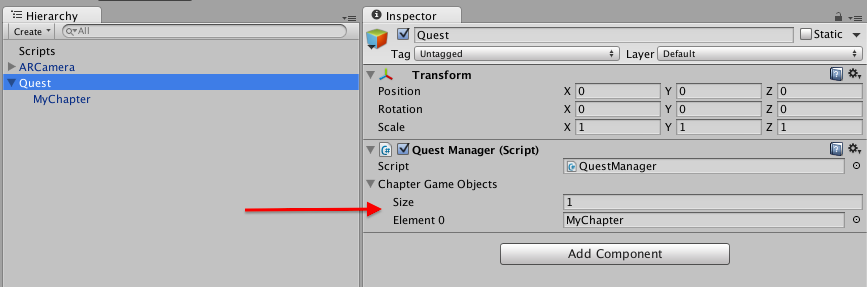
\includegraphics[width=0.9\textwidth]{figures/2-1.png}
\end{figure}
	
If you start the game now, you can see a new Chapter 1 button. Clicking on it leads to an empty chapter overview page. Here, the text description that leads to your location will be displayed.
	
Enter the texts into the fields in the inspector panel for the \textit{MyChapter} game object. There are two text fields for both pages in the journal. Note that the text has to be manually wrapped around the top right \textit{Camera} button.\\
	
The description that leads the players to the location should be accurate enough to find your location when starting from the last location. The player should be able to follow the directions and identify the right building facade where the puzzle is hidden. Players also have a compass available with the \textit{Compass} button, so you can use cardinal directions like north or south.\\
	
Also enter the GPS coordinates of your location in the corresponding fields. They are expected to be floats; Zurich is at 47.369317 latitude and 8.538775 longitude. This will be used in a help function during the game. Players who get lost can ask for the distance and direction to the next target.\\
	
The bottom two text fields are also used for the help function. There are two text hints for each puzzle which give small hints on how to solve the puzzle. Players can also skip the puzzles entirely if they get stuck however.\\
	
To test the help function, press the \textit{Help} button in the chapter overview. In this test view, all hints are unlocked by default whereas in the game, the hints are unlocked one by one.\\

\begin{figure}[H]
\centering
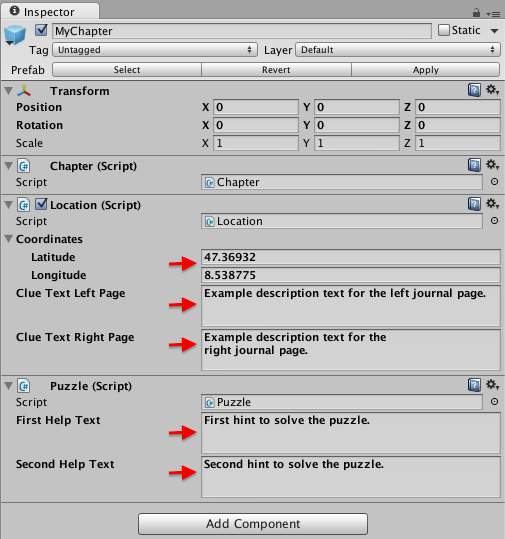
\includegraphics[width=0.9\textwidth]{figures/2-2.png}
\end{figure}

\textbf{3.}  Drag a \textit{MyPuzzle} prefab from the \textit{Prefabs} folder and set it up as a child of \textit{MyChapter}.\\

\textit{MyPuzzle} has one \textit{ImageTarget} as child per default. These are special objects provided by Vuforia. They contain the pictures that will be augmented with the puzzles. In this case a picture of a building facade. But for easier testing, we will use one of the default Vuforia markers for now. Set the data set to \textit{StonesAndChips} and the image target to \textit{stones} in the inspector.

\begin{figure}[H]
\centering
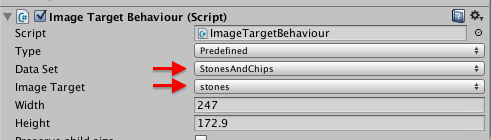
\includegraphics[width=0.9\textwidth]{figures/3-1.png}
\end{figure}

The three default markers \textit{stones}, \textit{chips} and \textit{tarmac} are provided in the \textit{VuforiaMarkers} pdf file. If you want to import your own data sets, do not forget to activate it in the inspector panel of the \textit{ARCamera} game object.\\

\begin{figure}[H]
\centering
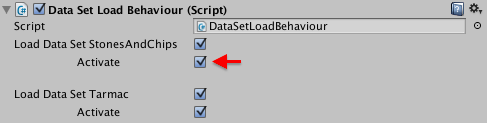
\includegraphics[width=0.9\textwidth]{figures/3-2.png}
\end{figure}

Our puzzle will be as simple as possible. It consists of one button that has to be pressed. The template includes buttons and levers to be used as puzzle elements. You can of course create your own components as well.\\

Drag a \textit{Button} prefab into the hierarchy and set it as child of the \textit{ImageTarget}. The button is built out of two models and has a \texttt{ButtonMovement} script attached which handles the animation. We only have to write a script which specifies what the button does when it is pressed.\\

Here is the complete hierarchy:

\begin{figure}[H]
\centering
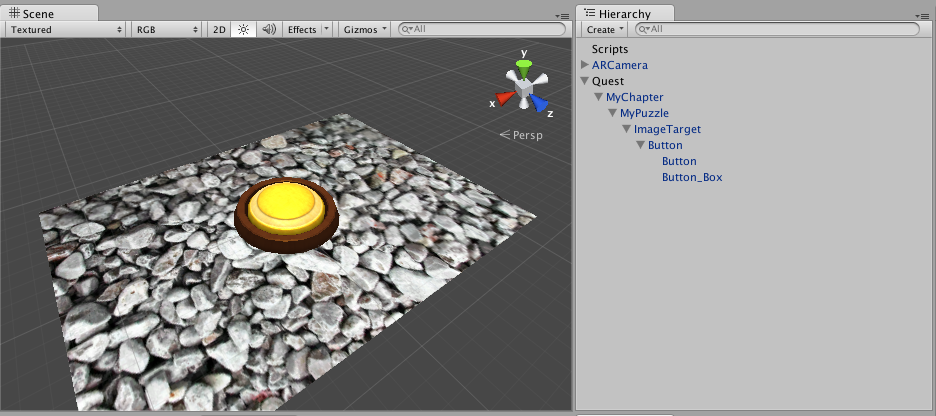
\includegraphics[width=0.9\textwidth]{figures/3-3.png}
\end{figure}

\textbf{4.} 

We will create two new scripts in the \textit{Scripts} folder to make the puzzle work. The first one is \texttt{MyButtonPuzzleLogic}, which inherits from the abstract class \texttt{PuzzleLogic}.\\

This script contains all data that is relevant to the puzzle, together with a public method to modify the data. In our example, we store whether the button was pressed in a boolean and provide the method \texttt{PressButton()} to change the value from outside.\\

There are two methods that have to be implemented: \texttt{CheckIfSolved()}, which checks the state of the data and returns whether the puzzle was solved and \texttt{Reset()}, which resets the data to the initial state. This happens at the start of the game and when the player starts a new game. \texttt{Reset()} should also reset all puzzle components that are attached. Levers that are pulled in the puzzle, for example, should be moved back to their start position so that the puzzle can be solved again.\\

There are also methods that are optional to implement: In \texttt{OnSolve()} and \texttt{OnSkip()} you can do clean up when a puzzle is solved or skipped. \texttt{OnUpdate()} works like a normal \texttt{Update()} method available in Unity scripts. It is called every frame and can be used for arbitrary code.\\

\lstinputlisting{code/MyButtonPuzzleLogic.cs}

The \texttt{MyButtonPuzzleLogic} script should be attached to the \textit{MyPuzzle} game object.\\

\begin{figure}[H]
\centering
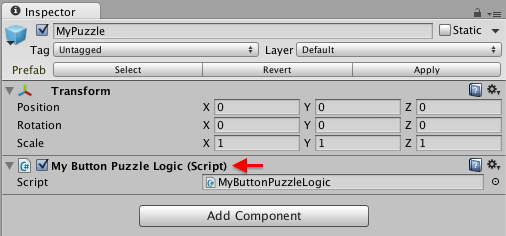
\includegraphics[width=0.9\textwidth]{figures/4-1.png}
\end{figure}

The second script is \texttt{MyButton}, which inherits from the \texttt{Button} class. It specifies what happens when the button is pressed in the \texttt{Action()} method that has to be implemented.\\

In our case, the \texttt{PressButton()} method in the \texttt{MyButtonPuzzleLogic} must be triggered, for which a reference to the \texttt{PuzzleLogic} is necessary.\\

\lstinputlisting{code/MyButton1.cs}

Note the \texttt{UnpressButton()} method at the end. After pressing the button, it stays in its pressed state until this method is called. It resets the button to its normal state where it can be pressed again.
It is useful to do this explicitly as you might want to wait for something to finish before it can be pressed again, such as playing a long sound file.\\

The \texttt{MyButton} script should be attached to the \textit{Button} game object. Then, drag the \textit{MyPuzzle} game object to the \textit{Button} inspector panel to set up the reference mentioned above.\\

\begin{figure}[H]
\centering
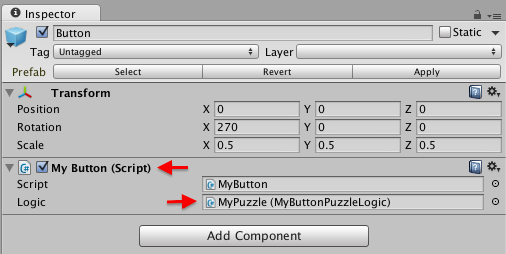
\includegraphics[width=0.9\textwidth]{figures/4-2.png}
\end{figure}

\textbf{5.} The puzzle should now be working. But let us also add a sound effect to the button.\\

Modify the \texttt{MyButton} script to include a \texttt{AudioClip} reference and add a line to the \texttt{Action()} method to play the sound in the main camera.\\

\lstinputlisting{code/MyButton2.cs}

Drag the sound effect \textit{Click} from the \textit{Sounds} folder to the \texttt{MyButton} inspector panel.\\

\begin{figure}[H]
\centering
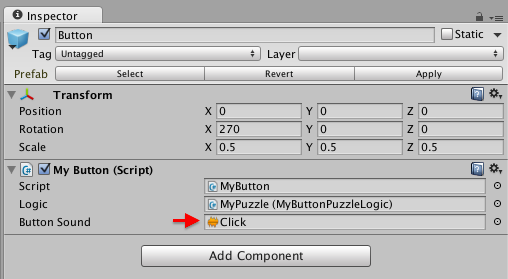
\includegraphics[width=0.9\textwidth]{figures/4-3.png}
\end{figure}

This completes our first puzzle.\\

To test it, run the game on a computer with a webcam or deploy the game on a mobile device with a camera. Navigate to Chapter 1, press the \textit{Camera} button and hold the \textit{stones} marker in front of the camera. You can use the mouse on a computer or touch input on a mobile device to press the button.\\

There are also the \textit{Skip} button for easy testing of the skip functionality in the game and the \textit{Reset} button to reset the puzzle to an unsolved state.

\section{Comments}

\textbf{Mouse and touch input}\\

To make input as easy as possible, an extension to the normal Unity \texttt{Transform} class is provided in the templates. Simply call \texttt{transform.IsTouched()} in a script attached to a game object to find out if it is touched. (This requires the game object to have a collider attached.)\\

\textbf{Disable input for buttons and levers}\\

The \texttt{Button} and \texttt{Lever} scripts also contain the methods \texttt{Activate()} and \texttt{Deactivate()} to enable and disable input.\\

\textbf{Levers}\\
	
Levers work very similar to buttons. As the model has two states however, they are a bit more complicated. Open the \textit{THTemplate2} Unity package in a new Unity project to see an example of a second chapter where the player has to pull a lever.\\
	
The \texttt{Lever} methods \texttt{SetToUpPosition()} and \texttt{SetToDownPosition()} are used in the \texttt{Reset()} and \texttt{OnSkip()} methods of \texttt{MyLeverPuzzleLogic} to move the lever down when the puzzle is skipped (to make it look like it was actually solved) and to move it back up when the game restarts. Note that this requires a \texttt{MyLever} reference in \texttt{MyLeverPuzzleLogic}.\\

Levers also have the methods \texttt{MoveToUpPosition()}, \texttt{MoveToDownPosition()}, which move the lever to its position with an animation and the two methods \texttt{IsMoving()} and \texttt{IsDown()} to find out whether the lever is currently moving and in which state it is.

\newpage


\end{document}